% !Mode:: "TeX:UTF-8"

\chapter{基于Boruvka算法和快速模糊C均值聚类的图像分割}

\begin{figure*}[h]
\begin{center}
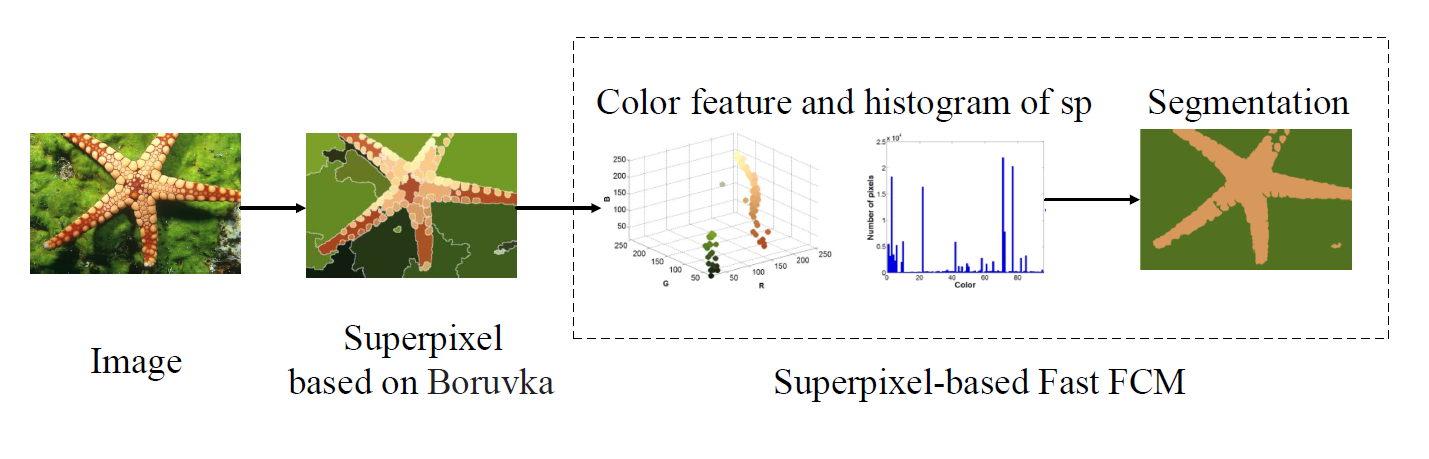
\includegraphics[width=1\textwidth]{figures/FCM2.png}
\end{center}
\vspace{-5mm}
\caption{算法流程图}
\label{fig4.1}
\end{figure*}

在这项工作中,我们使用一种基于Boruvka算法来产生超像素图像。Boruvka算法具有线性时间解,可并行化。此外,通过Boruvka 算法,得到连通分量。在每次迭代之后,元素特征在新形成的集群中进行聚合。这种方法比SLIC和LSC等只利用每个像素特征来确定聚类隶属关系的方法更为健壮。

在Boruvka算法获得的超像素图像的基础上,通过计算超像素图像的颜色直方图来实现快速模糊C 均值聚类。由于超像素图像中不同颜色的数目远小于原始彩色图像,因此计算超像素图像的颜色直方图非常容易。最后,以超像素颜色直方图作为目标函数的参数,实现彩色图像的快速分割。我们提出的算法的框架如图\ref{fig4.1}所示。

\section{基于Boruvka算法生成超像素}

把一个图看成有$n$个树的森林,每个顶点看成一棵树。
对于每棵树来说,我们找到它最近的邻点,即边的权重最小的那个点,并把他们合并在一起。
假设$C_{2}$是$C_{1}$的最小的邻点($C_{1}$也许并不是$C_{2}$最小的邻点),我们定义两个树之间的距离为:
\begin{equation}\label{eqn:hardassn}
D(C_{1},C_{2}) = \min_{v_{i}\in C_{1},v_{j}\in C_{2},(v_{i},v_{j})\in \varepsilon} \omega ((v_{i},v_{j}))
\end{equation}

最近邻点选择之后,构建辅助图,其中每个顶点表示一个簇,每个边对应一个选定的权重最小的边。如果这里有多个最近的邻点,我们在辅助图上用重复的边来表示他们。另一方面,辅助图上的边是不同的。用深度优先搜索找到连通图。Boruvka算法重复融合树直到只有一棵树留下来。我们用Boruvka算法生成一个最小生成树(MST),同时记录每个边缘的顺序添加到MST。一旦边缘被添加到MST,森林中的树木数量减少一个。假设需要提取$k$个超像素,我们通过前$n-k$个边连接顶点,并且具有$k$个连接的组件,这些组件恰好是超像素。

Boruvka和Kruskal算法之间的主要区别在于前者是局部和并发搜索边缘,而后者在全局范围内对边缘进行排序并按顺序执行。因此,Boruvka算法可以并行处理。此外,Boruvka算法假设簇是均匀分布的,并缓解了Kruskal算法倾向于生成严重不平衡簇的缺点。 在所提出的超像素层次方法中,我们采用Boruvka算法来构造MST。同时,记录每条边加入MST的顺序。一旦将一条边添加到MST中,森林中的树数将减少一棵。假设需要提取k个超像素,我们通过第一个n-k条边连接顶点,并且有k个连通的分量,这些分量就是超级像素。

\begin{figure*}[h]
\begin{center}
%\fbox{\rule{0pt}{2in} \rule{.9\linewidth}{0pt}}
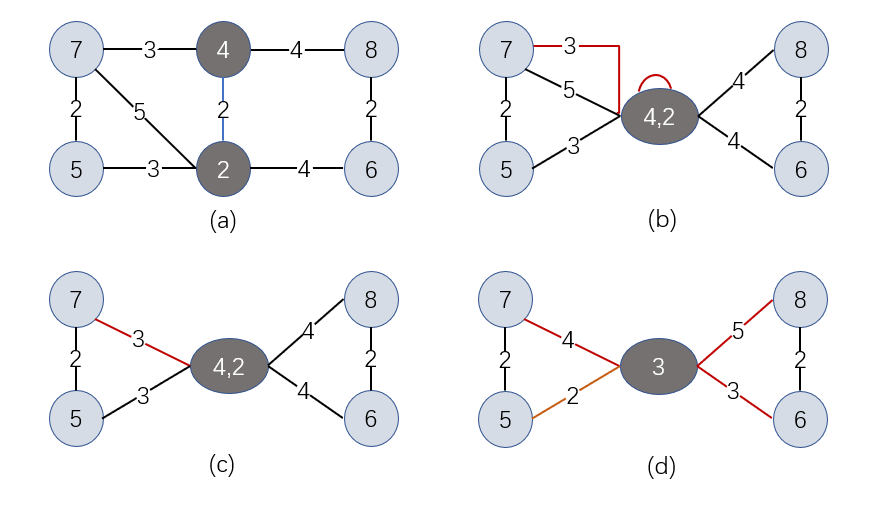
\includegraphics[width=1\textwidth]{figures/FCM1.png}
\end{center}
\vspace{-5mm}
\caption{边缘收缩和特征聚合。 每个顶点中的数字代表其特征值。 边缘权重通过其两端的绝对距离来计算。(a)-(c)在顶点4 和2之间执行边缘收缩。收缩边缘后,用自环替代收缩的边缘,并用平行边缘来保存原边的权重值。展平操作之后,移除自环并用权重较小的一条(红线)替换平行边缘。 (d)在每次迭代之后,通过从新形成的聚类中收集特征,然后更新边缘权重(红线)来进行特征聚合。}
\label{fig4.2}
\end{figure*}

Boruvka算法可以直接应用于超像素分割。然而,直接应用该算法并不能产生令人满意的结果。这些问题源于贪婪的局部算法设计,在计算最小边权重度量时,因为对于每棵树,只使用一个顶点的属性,所以对异常值很敏感。为了弥补这个缺陷,本方法对Boruvka 算法进行了改进,在同一个连通分量内合并邻域信息,称为边缘收缩。

边缘收缩如图\ref{fig4.2}所示。在图\ref{fig4.2}(a)的每个顶点,一个数字表示属性(例如,像素强度)。每个边权重由属性在两端的绝对距离计算。在顶点4和顶点2之间执行边收缩,形成一个超顶点。在图(c)中,保留较小的平行边。由于我们在每次迭代后都会得到新的簇,即新的连通分量,所以很自然地会聚集每个簇的属性并更新连接到其他簇的权重。
图\ref{fig4.2} (d)说明了这一过程。合并顶点4 和顶点2 后,将形成一个平均值为3 的超顶点。将删除自循环。同时,更新连接到超顶点的所有边的权重。特征聚合利用了“群体智慧”,而不是只利用两个顶点,这样可以获得更好的性能。

\section{基于超像素的快速模糊C均值聚类}
由于Boruvka算法依赖于图像的局部特征,而模糊C均值聚类依赖于全局特征,因此Boruvka算法和模糊C均值聚类的结合能够提高图像分割的效果。在这一部分中,我们提出了一种基于超像素的模糊C均值聚类算法,它将自适应的局部空间信息引入模糊C均值聚类的目标函数中。
\begin{equation}
J_{m} = \sum_{l=1}^{q}\sum_{k=1}^{c}S_{l}u_{kl}^{m} \left \| (\frac{1}{S_{l}}\sum_{p\in R_{l}}x_{p})-v_{k} \right \|^{2}
\end{equation}
其中,$l$是颜色级别,$1\leq l\leq q$,$q$是超像素图像的区域数量,即超像素数量,$S_{l}$是第$l$区域的像素数,$u_{kl}$ 表示颜色级别$l$相对于第$k$个聚类中心$v_{k}$的模糊隶属度,$m$为加权指数。$x_{p}$是超像素图像中第$l$区域内的颜色像素。由于原始图像中的每个颜色像素被超像素图像对应区域内的颜色像素的平均值所代替,所以颜色级别的数量相当于超级像素图像中的区域数量。因此,$l\ll N$,计算复杂度被有效地降低。

利用拉格朗日乘数法,将上述优化问题转化为一个无约束优化问题,该优化问题的目标函数为:
\begin{equation}
\widetilde{J_{m}} = \sum_{l=1}^{q}\sum_{k=1}^{c}S_{l}u_{kl}^{m} \left \| (\frac{1}{S_{l}}\sum_{p\in R_{l}}x_{p})-v_{k} \right \|^{2} - \lambda (\sum_{k=1}^{c}u_{kl}-1)
\end{equation}
其中$\lambda$是拉格朗日乘数。我们分别计算了$\widetilde{J_{m}}$关于$u_{kl}$和$v_k$的偏微分方程。

\begin{equation}
\begin{split}
\frac{\partial \widetilde{J_m}}{\partial u_{kl}}
&= \sum_{l=1}^{q}\sum_{k=1}^{c}\frac{\partial \sum_{l=1}^{q}\sum_{k=1}^{c}S_{l}u_{kl}^{m} \left \| (\frac{1}{S_{l}}\sum_{p\in R_{l}}x_{p})-v_{k} \right \|^{2}}{\partial u_{kl}}-\lambda \\
&= \sum_{l=1}^{q}\sum_{k=1}^{c}mS_{l}u_{m-1}^{kl}\left \| (\frac{1}{S_{l}}\sum_{p\in R_{l}}x_{p})-v_{k}  \right \|^{2} \\
&= 0
\end{split}
\label{eq4.4}
\end{equation}

\begin{equation}
\begin{split}
\frac{\partial \widetilde{J_m}}{\partial v_{k}}
&= \sum_{l=1}^{q}\sum_{k=1}^{c}\frac{\partial \sum_{l=1}^{q}\sum_{k=1}^{c}S_{l}u_{kl}^{m} \left \| (\frac{1}{S_{l}}\sum_{p\in R_{l}}x_{p})-v_{k} \right \|^{2}}{\partial v_{k}}  \\
&= \sum_{l=1}^{q}\sum_{k=1}^{c}S_{l}u_{m}^{kl}\frac{\partial \left \| (\frac{1}{S_{l}}\sum_{p\in R_{l}}x_{p})-v_{k}  \right \|^{2} }{\partial v_{k}} \\
&= \sum_{l=1}^{q} S_{l}u_{m}^{kl}\frac{\partial \left \| (\frac{1}{S_{l}}\sum_{p\in R_{l}}x_{p})-v_{k}  \right \|^{2} }{\partial v_{k}} \\
&= -2 \sum_{l=1}^{q} S_{l}u_{m}^{kl} \left \| (\frac{1}{S_{l}}\sum_{p\in R_{l}}x_{p})-v_{k} \right \| \\
&= 0
\end{split}
\label{eq4.5}
\end{equation}

将公式\ref{eq4.4}和公式\ref{eq4.5}结合起来,得到了$u_{kl}$和$v_k$的相应解:
\begin{equation}
v_{k} = \frac{\sum_{l=1}^{q} u_{kl}^{m} \sum_{p\in R_{l}} x_{p}}{\sum_{l=1}^{q} S_{l} u_{kl}^{m}}
\label{eq4.6}
\end{equation}

\begin{equation}
u_{kl} = \frac{ \left \| (\frac{1}{S_{l}}\sum_{p\in R_{l}}x_{p})-v_{k} \right \|^{-2/(m-1)} }
{ \sum_{j=1}^{c} \left \| (\frac{1}{S_{l}}\sum_{p\in R_{l}}x_{p})-v_{j} \right \|^{-2/(m-1)}}
\label{eq4.7}
\end{equation}

我们提出的算法可以总结如下:
\begin{itemize}
\item Step 1: 设置$c$, $m$,$\eta$的初始值, 其中$\eta$是我们算法的收敛条件。
\item Step 2: 根据超像素图像,随机初始化隶属度划分矩阵$U^{(0)}$。
\item Step 3: 设置循环计数器$b = 0$。
\item Step 4: 使用公式\ref{eq4.6}更新聚类中心。
\item Step 5: 使用公式\ref{eq4.7}更新隶属度划分矩阵$U^{(t)}$。
\item Step 6: 当$max{U^{(b)}-U^{(b+1)}}<\eta$,则停止;否则,设置$b=b+1$,跳转到步骤4。
\end{itemize}

\section{本章小结}

本章主要介绍了一种基于Boruvka算法和快速模糊C均值聚类的图像分割方法。
该方法首先使用基于Boruvka的算法来产生超像素。
在Boruvka算法获得的超像素图像的基础上,
通过计算超像素图像的颜色直方图来实现快速模糊C均值聚类,得到图像分割结果。